% Options for packages loaded elsewhere
\PassOptionsToPackage{unicode}{hyperref}
\PassOptionsToPackage{hyphens}{url}
%
\documentclass[
]{article}
\usepackage{amsmath,amssymb}
\usepackage{lmodern}
\usepackage{iftex}
\ifPDFTeX
  \usepackage[T1]{fontenc}
  \usepackage[utf8]{inputenc}
  \usepackage{textcomp} % provide euro and other symbols
\else % if luatex or xetex
  \usepackage{unicode-math}
  \defaultfontfeatures{Scale=MatchLowercase}
  \defaultfontfeatures[\rmfamily]{Ligatures=TeX,Scale=1}
\fi
% Use upquote if available, for straight quotes in verbatim environments
\IfFileExists{upquote.sty}{\usepackage{upquote}}{}
\IfFileExists{microtype.sty}{% use microtype if available
  \usepackage[]{microtype}
  \UseMicrotypeSet[protrusion]{basicmath} % disable protrusion for tt fonts
}{}
\makeatletter
\@ifundefined{KOMAClassName}{% if non-KOMA class
  \IfFileExists{parskip.sty}{%
    \usepackage{parskip}
  }{% else
    \setlength{\parindent}{0pt}
    \setlength{\parskip}{6pt plus 2pt minus 1pt}}
}{% if KOMA class
  \KOMAoptions{parskip=half}}
\makeatother
\usepackage{xcolor}
\usepackage[margin=1in]{geometry}
\usepackage{color}
\usepackage{fancyvrb}
\newcommand{\VerbBar}{|}
\newcommand{\VERB}{\Verb[commandchars=\\\{\}]}
\DefineVerbatimEnvironment{Highlighting}{Verbatim}{commandchars=\\\{\}}
% Add ',fontsize=\small' for more characters per line
\usepackage{framed}
\definecolor{shadecolor}{RGB}{248,248,248}
\newenvironment{Shaded}{\begin{snugshade}}{\end{snugshade}}
\newcommand{\AlertTok}[1]{\textcolor[rgb]{0.94,0.16,0.16}{#1}}
\newcommand{\AnnotationTok}[1]{\textcolor[rgb]{0.56,0.35,0.01}{\textbf{\textit{#1}}}}
\newcommand{\AttributeTok}[1]{\textcolor[rgb]{0.77,0.63,0.00}{#1}}
\newcommand{\BaseNTok}[1]{\textcolor[rgb]{0.00,0.00,0.81}{#1}}
\newcommand{\BuiltInTok}[1]{#1}
\newcommand{\CharTok}[1]{\textcolor[rgb]{0.31,0.60,0.02}{#1}}
\newcommand{\CommentTok}[1]{\textcolor[rgb]{0.56,0.35,0.01}{\textit{#1}}}
\newcommand{\CommentVarTok}[1]{\textcolor[rgb]{0.56,0.35,0.01}{\textbf{\textit{#1}}}}
\newcommand{\ConstantTok}[1]{\textcolor[rgb]{0.00,0.00,0.00}{#1}}
\newcommand{\ControlFlowTok}[1]{\textcolor[rgb]{0.13,0.29,0.53}{\textbf{#1}}}
\newcommand{\DataTypeTok}[1]{\textcolor[rgb]{0.13,0.29,0.53}{#1}}
\newcommand{\DecValTok}[1]{\textcolor[rgb]{0.00,0.00,0.81}{#1}}
\newcommand{\DocumentationTok}[1]{\textcolor[rgb]{0.56,0.35,0.01}{\textbf{\textit{#1}}}}
\newcommand{\ErrorTok}[1]{\textcolor[rgb]{0.64,0.00,0.00}{\textbf{#1}}}
\newcommand{\ExtensionTok}[1]{#1}
\newcommand{\FloatTok}[1]{\textcolor[rgb]{0.00,0.00,0.81}{#1}}
\newcommand{\FunctionTok}[1]{\textcolor[rgb]{0.00,0.00,0.00}{#1}}
\newcommand{\ImportTok}[1]{#1}
\newcommand{\InformationTok}[1]{\textcolor[rgb]{0.56,0.35,0.01}{\textbf{\textit{#1}}}}
\newcommand{\KeywordTok}[1]{\textcolor[rgb]{0.13,0.29,0.53}{\textbf{#1}}}
\newcommand{\NormalTok}[1]{#1}
\newcommand{\OperatorTok}[1]{\textcolor[rgb]{0.81,0.36,0.00}{\textbf{#1}}}
\newcommand{\OtherTok}[1]{\textcolor[rgb]{0.56,0.35,0.01}{#1}}
\newcommand{\PreprocessorTok}[1]{\textcolor[rgb]{0.56,0.35,0.01}{\textit{#1}}}
\newcommand{\RegionMarkerTok}[1]{#1}
\newcommand{\SpecialCharTok}[1]{\textcolor[rgb]{0.00,0.00,0.00}{#1}}
\newcommand{\SpecialStringTok}[1]{\textcolor[rgb]{0.31,0.60,0.02}{#1}}
\newcommand{\StringTok}[1]{\textcolor[rgb]{0.31,0.60,0.02}{#1}}
\newcommand{\VariableTok}[1]{\textcolor[rgb]{0.00,0.00,0.00}{#1}}
\newcommand{\VerbatimStringTok}[1]{\textcolor[rgb]{0.31,0.60,0.02}{#1}}
\newcommand{\WarningTok}[1]{\textcolor[rgb]{0.56,0.35,0.01}{\textbf{\textit{#1}}}}
\usepackage{graphicx}
\makeatletter
\def\maxwidth{\ifdim\Gin@nat@width>\linewidth\linewidth\else\Gin@nat@width\fi}
\def\maxheight{\ifdim\Gin@nat@height>\textheight\textheight\else\Gin@nat@height\fi}
\makeatother
% Scale images if necessary, so that they will not overflow the page
% margins by default, and it is still possible to overwrite the defaults
% using explicit options in \includegraphics[width, height, ...]{}
\setkeys{Gin}{width=\maxwidth,height=\maxheight,keepaspectratio}
% Set default figure placement to htbp
\makeatletter
\def\fps@figure{htbp}
\makeatother
\setlength{\emergencystretch}{3em} % prevent overfull lines
\providecommand{\tightlist}{%
  \setlength{\itemsep}{0pt}\setlength{\parskip}{0pt}}
\setcounter{secnumdepth}{5}
\ifLuaTeX
  \usepackage{selnolig}  % disable illegal ligatures
\fi
\IfFileExists{bookmark.sty}{\usepackage{bookmark}}{\usepackage{hyperref}}
\IfFileExists{xurl.sty}{\usepackage{xurl}}{} % add URL line breaks if available
\urlstyle{same} % disable monospaced font for URLs
\hypersetup{
  pdftitle={Taller 2 Regresión lineal Multiple},
  pdfauthor={Andrés Felipe Palomino - David Stiven Rojas},
  hidelinks,
  pdfcreator={LaTeX via pandoc}}

\title{Taller 2 Regresión lineal Multiple}
\author{Andrés Felipe Palomino - David Stiven Rojas}
\date{2023-04-21}

\begin{document}
\maketitle

\hypertarget{introducciuxf3n}{%
\section{Introducción}\label{introducciuxf3n}}

La base de datos \("yarn"\) obtenida de la librería (PLS) contiene
información sobre espectros NIR y mediciones de densidad de hilos de
PET, consta de 28 individuos (hilos de PET), 268 variables predictoras
(NIRS) y una variable de respuesta (densidad). Se ajustará un modelo
lineal múltiple para estimar la densidad del hilo PET, mediante
mediciones NIR

\begin{Shaded}
\begin{Highlighting}[]
\CommentTok{\#Importación de librerías necesarias}
\FunctionTok{library}\NormalTok{(car)}
\FunctionTok{library}\NormalTok{(glmnet)}
\FunctionTok{library}\NormalTok{(MASS)}
\FunctionTok{library}\NormalTok{(xtable)}
\FunctionTok{library}\NormalTok{(lmtest)}
\FunctionTok{library}\NormalTok{(readxl)}
\FunctionTok{library}\NormalTok{(lmridge)}
\FunctionTok{library}\NormalTok{(pls)}
\FunctionTok{library}\NormalTok{(olsrr)}
\end{Highlighting}
\end{Shaded}

\hypertarget{base-de-datos}{%
\subsection{Base de datos}\label{base-de-datos}}

En la siguiente tabla se encuentra un encabezado de la base de datos que
se trabajara, esta consta de 30 covariables predictoras, las cuales
estarán desde NIR1 hasta NIR30. De primera mano se observa que los
valores de los NIR disminuyen a medida que la covariable aumenta

\begin{Shaded}
\begin{Highlighting}[]
\NormalTok{X }\OtherTok{\textless{}{-}} \FunctionTok{data.frame}\NormalTok{(}\FunctionTok{matrix}\NormalTok{(}\FunctionTok{c}\NormalTok{(yarn}\SpecialCharTok{$}\NormalTok{NIR[,}\DecValTok{1}\SpecialCharTok{:}\DecValTok{30}\NormalTok{],yarn}\SpecialCharTok{$}\NormalTok{density),}\AttributeTok{nrow =}\DecValTok{28}\NormalTok{, }\AttributeTok{ncol=} \DecValTok{31}\NormalTok{))}
\FunctionTok{colnames}\NormalTok{(X) }\OtherTok{\textless{}{-}} \FunctionTok{c}\NormalTok{(}\FunctionTok{paste}\NormalTok{(}\StringTok{"NIR"}\NormalTok{,}\DecValTok{1}\SpecialCharTok{:}\DecValTok{30}\NormalTok{,}\AttributeTok{sep=}\StringTok{""}\NormalTok{),}\StringTok{"density"}\NormalTok{)}
\end{Highlighting}
\end{Shaded}

\hypertarget{funciones-creadas}{%
\subsection{Funciones creadas}\label{funciones-creadas}}

Antes de empezar con el proceso de seleccionar las variables para
ajustar el modelo se crean funciones para optimizar el proceso de
validación de supuestos, debido a que constantemente se deben realizar,
estas funciones estan diseñadas para objetos lm.

\begin{Shaded}
\begin{Highlighting}[]
\DocumentationTok{\#\#Validacion grafica para homocedasticidad y normalidad y pruebas formales}
\NormalTok{validaciongrafica}\OtherTok{\textless{}{-}} \ControlFlowTok{function}\NormalTok{(model,}\AttributeTok{cor=}\NormalTok{F)\{}
  
  \FunctionTok{par}\NormalTok{(}\AttributeTok{mfrow=}\FunctionTok{c}\NormalTok{(}\DecValTok{1}\NormalTok{,}\DecValTok{2}\NormalTok{))}
  \FunctionTok{plot}\NormalTok{(}\FunctionTok{fitted.values}\NormalTok{(model),}\FunctionTok{studres}\NormalTok{(model),}\AttributeTok{panel.first=}\FunctionTok{grid}\NormalTok{(),}
       \AttributeTok{pch=}\DecValTok{19}\NormalTok{,}\AttributeTok{ylab=}\StringTok{\textquotesingle{}Residuos Estudentizados\textquotesingle{}}\NormalTok{,}\AttributeTok{xlab=}\StringTok{\textquotesingle{}Valores ajustados\textquotesingle{}}\NormalTok{,}\AttributeTok{main=}\StringTok{\textquotesingle{}A\textquotesingle{}}\NormalTok{,}\AttributeTok{col=}\StringTok{\textquotesingle{}aquamarine4\textquotesingle{}}\NormalTok{)}
  \FunctionTok{abline}\NormalTok{(}\AttributeTok{h=}\FunctionTok{c}\NormalTok{(}\SpecialCharTok{{-}}\DecValTok{2}\NormalTok{,}\DecValTok{0}\NormalTok{,}\DecValTok{2}\NormalTok{),}\AttributeTok{lty=}\DecValTok{2}\NormalTok{)}
  \FunctionTok{qqPlot}\NormalTok{(model,}\AttributeTok{pch=}\DecValTok{19}\NormalTok{,}\AttributeTok{ylab=}\StringTok{\textquotesingle{}Residuos Estudentizados\textquotesingle{}}\NormalTok{,}
         \AttributeTok{xlab=}\StringTok{\textquotesingle{}Cuantiles Teóricos\textquotesingle{}}\NormalTok{,}\AttributeTok{col=}\FunctionTok{carPalette}\NormalTok{()[}\DecValTok{1}\NormalTok{],}
         \AttributeTok{col.lines=}\FunctionTok{carPalette}\NormalTok{()[}\DecValTok{3}\NormalTok{],}\AttributeTok{main=}\StringTok{\textquotesingle{}B\textquotesingle{}}\NormalTok{)}
  \FunctionTok{print}\NormalTok{(}\StringTok{\textquotesingle{}Shapiro Test; H0: Normalidad vs H1: No Normalidad\textquotesingle{}}\NormalTok{)}
  \FunctionTok{print}\NormalTok{(}\FunctionTok{shapiro.test}\NormalTok{(}\FunctionTok{studres}\NormalTok{(model)))}
  \FunctionTok{print}\NormalTok{(}\StringTok{\textquotesingle{}Breusch Pagan Test;H0: Homocedasticidad vs H1: No Homocedasticidad\textquotesingle{}}\NormalTok{)}
  \FunctionTok{print}\NormalTok{(}\FunctionTok{bptest}\NormalTok{(model))}
  \ControlFlowTok{if}\NormalTok{(cor}\SpecialCharTok{==}\NormalTok{T)\{}
    \FunctionTok{par}\NormalTok{(}\AttributeTok{mfrow=}\FunctionTok{c}\NormalTok{(}\DecValTok{1}\NormalTok{,}\DecValTok{2}\NormalTok{))}
    \FunctionTok{plot}\NormalTok{(}\FunctionTok{studres}\NormalTok{(model),}\AttributeTok{type=}\StringTok{"b"}\NormalTok{,}\AttributeTok{xlab=}\StringTok{"Tiempo"}\NormalTok{,}\AttributeTok{ylab=}\StringTok{"Residuos Estudentizados"}\NormalTok{,}\AttributeTok{main=}\StringTok{"A"}\NormalTok{,}
         \AttributeTok{pch=}\DecValTok{19}\NormalTok{,}\AttributeTok{panel.first=}\FunctionTok{grid}\NormalTok{())}
    \FunctionTok{plot}\NormalTok{(}\FunctionTok{studres}\NormalTok{(model)[}\SpecialCharTok{{-}}\FunctionTok{length}\NormalTok{(}\FunctionTok{fitted.values}\NormalTok{(model))],}
         \FunctionTok{studres}\NormalTok{(model)[}\SpecialCharTok{{-}}\DecValTok{1}\NormalTok{],}\AttributeTok{pch=}\DecValTok{19}\NormalTok{,}\AttributeTok{panel.first =} \FunctionTok{grid}\NormalTok{(),}\AttributeTok{col=}\StringTok{"turquoise3"}\NormalTok{,}
         \AttributeTok{xlab=}\FunctionTok{TeX}\NormalTok{(}\StringTok{"$Residuos\_\{t{-}1\}$"}\NormalTok{),}\AttributeTok{ylab=}\FunctionTok{TeX}\NormalTok{(}\StringTok{"$Residuos\_\{t\}$"}\NormalTok{),}\AttributeTok{main=}\StringTok{"B"}\NormalTok{)}
    \FunctionTok{abline}\NormalTok{(}\FunctionTok{lm}\NormalTok{(}\FunctionTok{studres}\NormalTok{(model)[}\SpecialCharTok{{-}}\DecValTok{1}\NormalTok{]}\SpecialCharTok{\textasciitilde{}}\FunctionTok{studres}\NormalTok{(model)[}\SpecialCharTok{{-}}\FunctionTok{length}\NormalTok{(}\FunctionTok{fitted.values}\NormalTok{(model))]))}
    \FunctionTok{print}\NormalTok{(}\StringTok{\textquotesingle{}Durbin Watson Test\textquotesingle{}}\NormalTok{)}
    \FunctionTok{print}\NormalTok{(}\FunctionTok{durbinWatsonTest}\NormalTok{(model,}
                           \AttributeTok{method=}\StringTok{\textquotesingle{}resample\textquotesingle{}}\NormalTok{,}\AttributeTok{reps=}\DecValTok{10000}\NormalTok{))}
\NormalTok{  \}}
  \FunctionTok{par}\NormalTok{(}\AttributeTok{mfrow=}\FunctionTok{c}\NormalTok{(}\DecValTok{1}\NormalTok{,}\DecValTok{1}\NormalTok{))}
\NormalTok{\}}

\DocumentationTok{\#\# Calculo de lambda optimo para boxcox}
\NormalTok{lambda}\OtherTok{\textless{}{-}} \ControlFlowTok{function}\NormalTok{(model,a,b)\{}
  \FunctionTok{par}\NormalTok{(}\AttributeTok{mfrow=}\FunctionTok{c}\NormalTok{(}\DecValTok{1}\NormalTok{,}\DecValTok{1}\NormalTok{))}
\NormalTok{  box.cox}\OtherTok{\textless{}{-}}\FunctionTok{boxcox}\NormalTok{(model,}\AttributeTok{lambda=}\FunctionTok{seq}\NormalTok{(a,b,}\AttributeTok{length.out =} \DecValTok{1000}\NormalTok{),}
                  \AttributeTok{ylab=}\StringTok{\textquotesingle{}log{-}verosimilitud\textquotesingle{}}\NormalTok{)}
\NormalTok{  bc}\OtherTok{\textless{}{-}}\FunctionTok{round}\NormalTok{(box.cox}\SpecialCharTok{$}\NormalTok{x[box.cox}\SpecialCharTok{$}\NormalTok{y }\SpecialCharTok{==}\FunctionTok{max}\NormalTok{(box.cox}\SpecialCharTok{$}\NormalTok{y)],}\DecValTok{2}\NormalTok{)}
  \FunctionTok{print}\NormalTok{(bc)}
\NormalTok{\}}
\end{Highlighting}
\end{Shaded}

\hypertarget{selecciuxf3n-de-variables}{%
\section{Selección de variables}\label{selecciuxf3n-de-variables}}

En el proceso de selección de variables se procede a realizar la
Regresion de LASSO para identificar las posibles variables que tengan un
aporte poco relevante, Por ultimo se ajustara el modelo cuyas variables
tengan buenos indicadores y se pueda realizar corrección de supuestos

\hypertarget{regresiuxf3n-de-lasso}{%
\subsection{Regresión de LASSO}\label{regresiuxf3n-de-lasso}}

Este es un método de regularización que se implementa cuando se tiene
muchas covariables disponibles y se cree que pocas tienen un aporte
relevante.

Se asume el modelo de regresión usual, donde :

\begin{center}
E(y|x)=$X^T\beta$, y V(y|x)=$\sigma^2$
\end{center}

Donde se asume que algunos \(\beta\) son cero. El objetivo del estimador
es seleccionar los coeficientes que tienen valores diferentes de cero.
El cual se obtiene minimizando la siguiente expresión:

\begin{center}
$S_{lasso}(\beta)=\sum_{i=1}^{n}({y_{i}-x^
T}\beta)^2+\lambda\sum_{j=1}^{p-1}|\beta_{j}|$
\end{center}

Esta es la suma de cuadrados del estimador por MCO más una penalización
(\(\lambda\)), a la suma del valor absoluto de los coeficientes. A
medida que \(\lambda\) aumenta la penalización tendrá mas peso sobre la
estimación de los coeficientes, es decir que si la penalización es muy
grande, todas las estimaciones seran cero. No hay solución analitica
para \(\hat{\beta}_{lasso}\) por lo que se usan algoritmos para la
estimación, como lo es la funcion de glmnet de la libreria glmnet.

\hypertarget{modelo-a-realizar-regresiuxf3n-lasso}{%
\subsubsection{Modelo a realizar regresión
LASSO}\label{modelo-a-realizar-regresiuxf3n-lasso}}

Como se establecio anteriormente, se asume un modelo de regresión usual,
el cual debe cumplir los siguientes supuestos:
E(y\textbar x)=\(x^T\beta\), y V(y\textbar x)=\(\sigma^2\), es decir,
varianza constante y E(\(\varepsilon\))=0 . Por ende es necesario
proponer un modelo con p\textless n, en el cual se eliminaran las
variables con menor correlación con la variable density. Dicho modelo se
expresa acontinuación y se evaluan los supuestos:

\begin{Shaded}
\begin{Highlighting}[]
\NormalTok{model }\OtherTok{\textless{}{-}} \FunctionTok{lm}\NormalTok{(density }\SpecialCharTok{\textasciitilde{}}\NormalTok{ .}\SpecialCharTok{{-}}\NormalTok{NIR1}\SpecialCharTok{{-}}\NormalTok{NIR8}\SpecialCharTok{{-}}\NormalTok{NIR9}\SpecialCharTok{{-}}\NormalTok{NIR10}\SpecialCharTok{{-}}\NormalTok{NIR11}\SpecialCharTok{{-}}\NormalTok{NIR7, }\AttributeTok{data=}\NormalTok{X)}
\NormalTok{car}\SpecialCharTok{::}\FunctionTok{vif}\NormalTok{(model)[}\DecValTok{1}\SpecialCharTok{:}\DecValTok{5}\NormalTok{]}
\end{Highlighting}
\end{Shaded}

\begin{verbatim}
##       NIR2       NIR3       NIR4       NIR5       NIR6 
##   1664.742  39841.316 361180.516 623252.841 254014.085
\end{verbatim}

\begin{Shaded}
\begin{Highlighting}[]
\NormalTok{car}\SpecialCharTok{::}\FunctionTok{vif}\NormalTok{(model)[}\DecValTok{6}\SpecialCharTok{:}\DecValTok{10}\NormalTok{]}
\end{Highlighting}
\end{Shaded}

\begin{verbatim}
##    NIR12    NIR13    NIR14    NIR15    NIR16 
##  8859706 76280654 79779619 53664079 80678703
\end{verbatim}

\begin{Shaded}
\begin{Highlighting}[]
\NormalTok{car}\SpecialCharTok{::}\FunctionTok{vif}\NormalTok{(model)[}\DecValTok{11}\SpecialCharTok{:}\DecValTok{16}\NormalTok{]}
\end{Highlighting}
\end{Shaded}

\begin{verbatim}
##     NIR17     NIR18     NIR19     NIR20     NIR21     NIR22 
##  99398953 163539741 308758563 360036341 277176909 369337378
\end{verbatim}

\begin{Shaded}
\begin{Highlighting}[]
\NormalTok{car}\SpecialCharTok{::}\FunctionTok{vif}\NormalTok{(model)[}\DecValTok{17}\SpecialCharTok{:}\DecValTok{24}\NormalTok{]}
\end{Highlighting}
\end{Shaded}

\begin{verbatim}
##     NIR23     NIR24     NIR25     NIR26     NIR27     NIR28     NIR29     NIR30 
## 475476287 461114938 385039631 205007476  70428412  37122355  20001842   1522304
\end{verbatim}

\begin{Shaded}
\begin{Highlighting}[]
\FunctionTok{validaciongrafica}\NormalTok{(model)}
\end{Highlighting}
\end{Shaded}

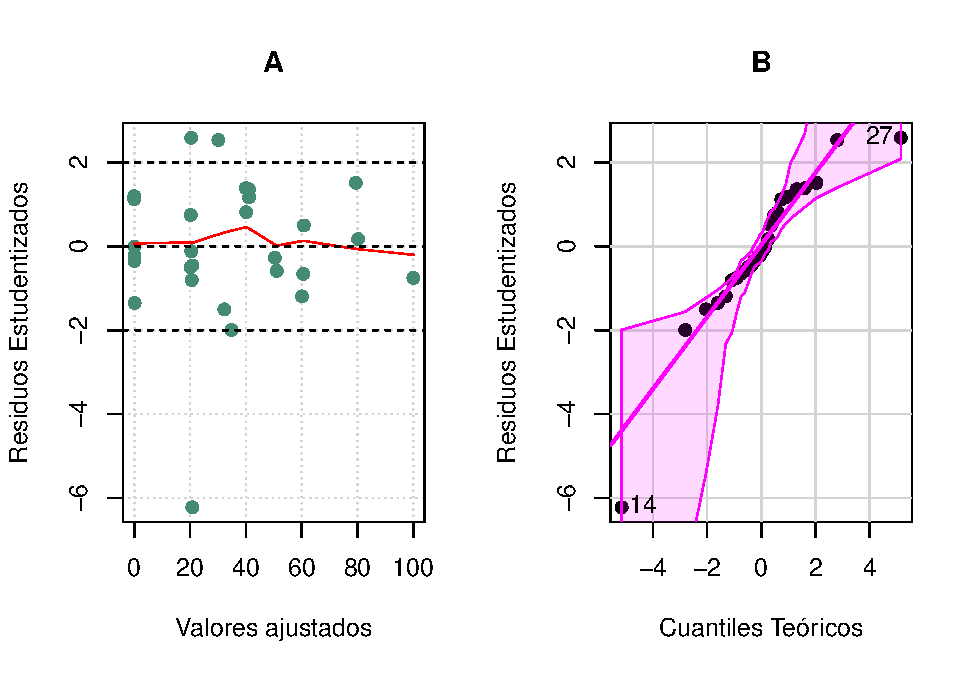
\includegraphics{Taller-2-Regresion-Multiple-Aplicada_files/figure-latex/unnamed-chunk-4-1.pdf}

\begin{verbatim}
## [1] "Shapiro Test; H0: Normalidad vs H1: No Normalidad"
## 
##  Shapiro-Wilk normality test
## 
## data:  studres(model)
## W = 0.86458, p-value = 0.001868
## 
## [1] "Breusch Pagan Test;H0: Homocedasticidad vs H1: No Homocedasticidad"
## 
##  studentized Breusch-Pagan test
## 
## data:  model
## BP = 27.288, df = 24, p-value = 0.2912
\end{verbatim}

Mediante el grafico y los valores P asociados a la homocedasticidad y
normalidad de residuos se evidencia el incumplimiento de la normalidad
de los residuos.

\begin{Shaded}
\begin{Highlighting}[]
\FunctionTok{hist}\NormalTok{(}\FunctionTok{studres}\NormalTok{(model),}\AttributeTok{lwd=}\DecValTok{2}\NormalTok{,}\AttributeTok{col=}\StringTok{\textquotesingle{}aquamarine4\textquotesingle{}}\NormalTok{,}\AttributeTok{freq=}\NormalTok{F,}\AttributeTok{ylim=}\FunctionTok{c}\NormalTok{(}\DecValTok{0}\NormalTok{,}\FloatTok{0.4}\NormalTok{),}
     \AttributeTok{xlab=}\StringTok{\textquotesingle{}Residuos Estudentizados Modelo\textquotesingle{}}\NormalTok{,}\AttributeTok{main=}\StringTok{\textquotesingle{}\textquotesingle{}}\NormalTok{)}
\FunctionTok{lines}\NormalTok{(}\FunctionTok{density}\NormalTok{(}\FunctionTok{studres}\NormalTok{(model)),}\AttributeTok{lwd=}\DecValTok{2}\NormalTok{,}\AttributeTok{col=}\StringTok{\textquotesingle{}black\textquotesingle{}}\NormalTok{)}
\end{Highlighting}
\end{Shaded}

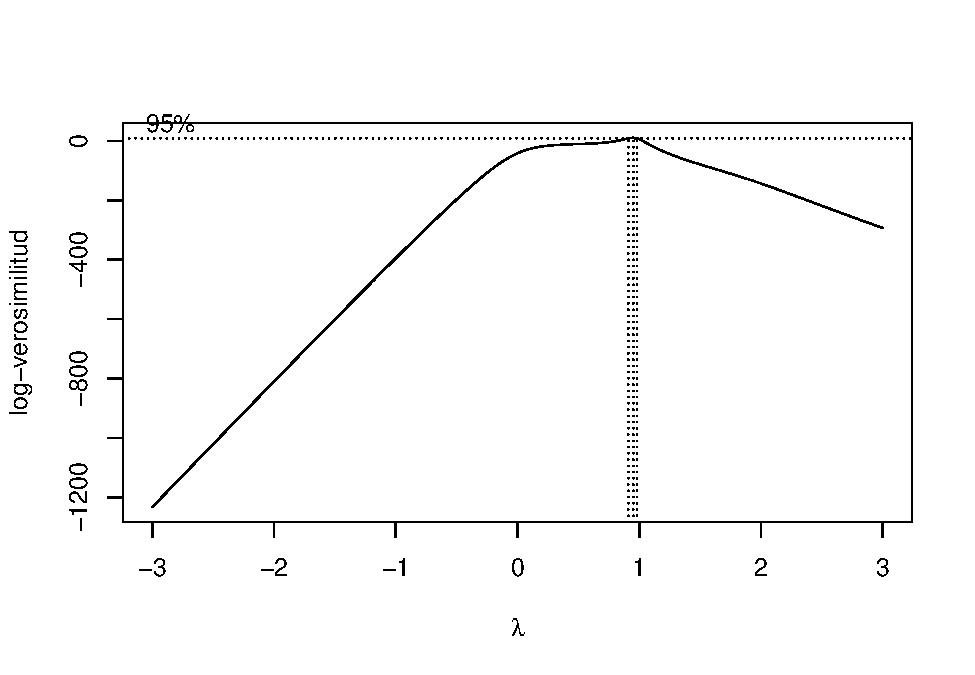
\includegraphics{Taller-2-Regresion-Multiple-Aplicada_files/figure-latex/unnamed-chunk-5-1.pdf}

Como no se cumple el supuesto de normalidad se procede a corregir
mediante el metodo de BoxCox y se verifica el cumplimiento de los
mismos.

\begin{Shaded}
\begin{Highlighting}[]
\NormalTok{model }\OtherTok{\textless{}{-}} \FunctionTok{lm}\NormalTok{(density}\FloatTok{+0.01} \SpecialCharTok{\textasciitilde{}}\NormalTok{ .}\SpecialCharTok{{-}}\NormalTok{NIR1}\SpecialCharTok{{-}}\NormalTok{NIR8}\SpecialCharTok{{-}}\NormalTok{NIR9}\SpecialCharTok{{-}}\NormalTok{NIR10}\SpecialCharTok{{-}}\NormalTok{NIR11}\SpecialCharTok{{-}}\NormalTok{NIR7, }\AttributeTok{data=}\NormalTok{X)}
\FunctionTok{lambda}\NormalTok{(model,}\FloatTok{0.5}\NormalTok{,}\FloatTok{1.5}\NormalTok{)}
\end{Highlighting}
\end{Shaded}

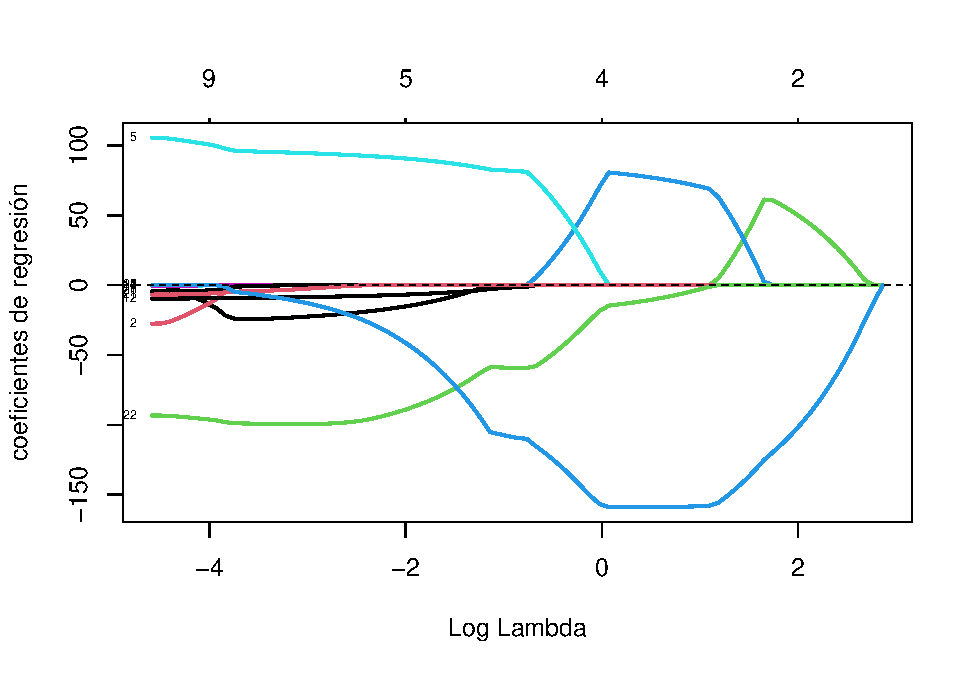
\includegraphics{Taller-2-Regresion-Multiple-Aplicada_files/figure-latex/unnamed-chunk-6-1.pdf}

\begin{verbatim}
## [1] 0.97
\end{verbatim}

\begin{Shaded}
\begin{Highlighting}[]
\NormalTok{model.box }\OtherTok{\textless{}{-}} \FunctionTok{lm}\NormalTok{(}\FunctionTok{I}\NormalTok{(density}\SpecialCharTok{\^{}}\FloatTok{0.96}\NormalTok{) }\SpecialCharTok{\textasciitilde{}}\NormalTok{.}\SpecialCharTok{{-}}\NormalTok{NIR1}\SpecialCharTok{{-}}\NormalTok{NIR8}\SpecialCharTok{{-}}\NormalTok{NIR9}\SpecialCharTok{{-}}\NormalTok{NIR10}\SpecialCharTok{{-}}\NormalTok{NIR11}\SpecialCharTok{{-}}\NormalTok{NIR7,}\AttributeTok{data=}\NormalTok{X)}
\FunctionTok{validaciongrafica}\NormalTok{(model.box)}
\end{Highlighting}
\end{Shaded}

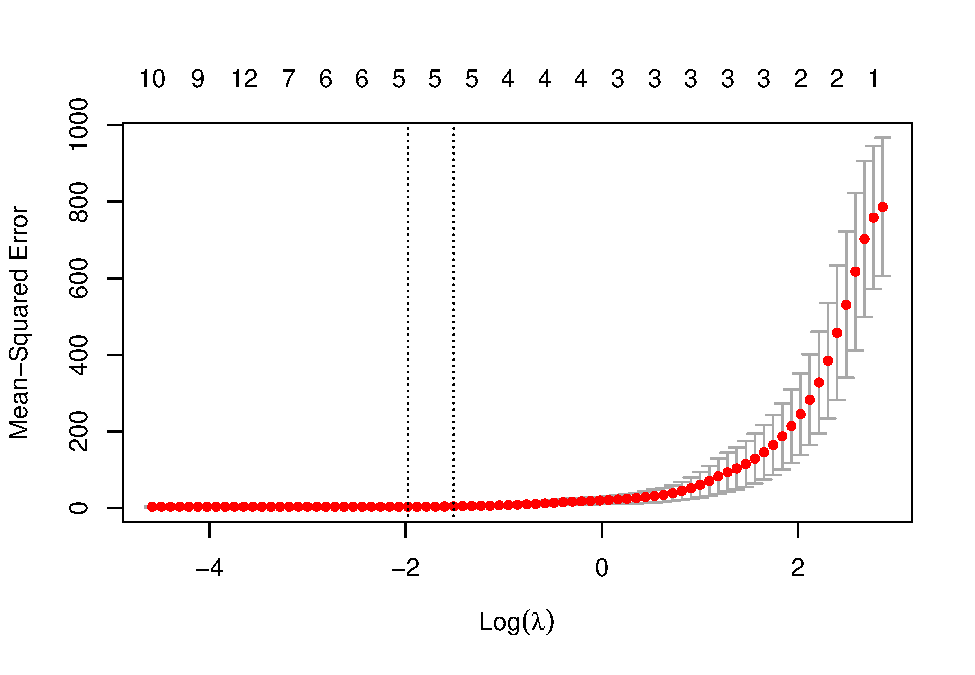
\includegraphics{Taller-2-Regresion-Multiple-Aplicada_files/figure-latex/unnamed-chunk-7-1.pdf}
{[}1{]} ``Shapiro Test; H0: Normalidad vs H1: No Normalidad''

\begin{verbatim}
Shapiro-Wilk normality test
\end{verbatim}

data: studres(model) W = 0.97774, p-value = 0.7934

{[}1{]} ``Breusch Pagan Test;H0: Homocedasticidad vs H1: No
Homocedasticidad''

\begin{verbatim}
studentized Breusch-Pagan test
\end{verbatim}

data: model BP = 23.94, df = 24, p-value = 0.4651

Mediante el grafico y los valores P asociados a la homocedasticidad y
normalidad de residuos se evidencia el cumplimiento de ambos supuestos.

\begin{Shaded}
\begin{Highlighting}[]
\FunctionTok{hist}\NormalTok{(}\FunctionTok{studres}\NormalTok{(model.box),}\AttributeTok{lwd=}\DecValTok{2}\NormalTok{,}\AttributeTok{col=}\StringTok{\textquotesingle{}aquamarine4\textquotesingle{}}\NormalTok{,}
\AttributeTok{freq=}\NormalTok{F,}\AttributeTok{ylim=}\FunctionTok{c}\NormalTok{(}\DecValTok{0}\NormalTok{,}\FloatTok{0.4}\NormalTok{),}\AttributeTok{xlab=}\StringTok{\textquotesingle{}Residuos Estudentizados Modelo\textquotesingle{}}\NormalTok{,}\AttributeTok{main=}\StringTok{\textquotesingle{}\textquotesingle{}}\NormalTok{)}
\FunctionTok{lines}\NormalTok{(}\FunctionTok{density}\NormalTok{(}\FunctionTok{studres}\NormalTok{(model.box)),}\AttributeTok{lwd=}\DecValTok{2}\NormalTok{,}\AttributeTok{col=}\StringTok{\textquotesingle{}black\textquotesingle{}}\NormalTok{)}
\end{Highlighting}
\end{Shaded}

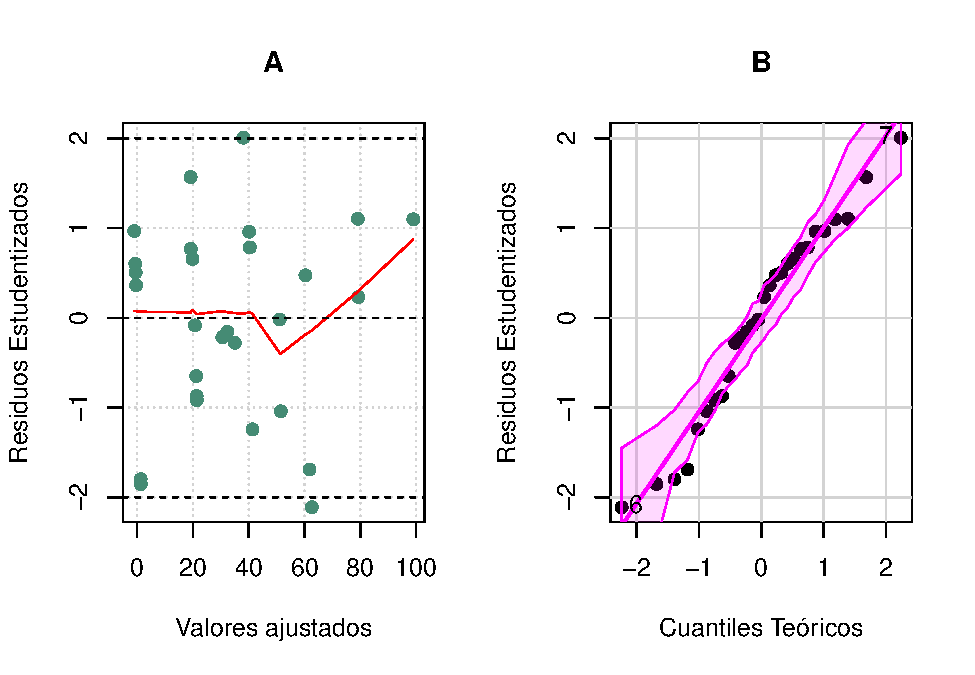
\includegraphics{Taller-2-Regresion-Multiple-Aplicada_files/figure-latex/unnamed-chunk-8-1.pdf}

Ya con los requerimentos necesarios para realizar regresión de LASSO se
procede a calcular el valor de \(\lambda\) optimo mediante la validación
cruzada

\hypertarget{validaciuxf3n-cruzada}{%
\subsubsection{Validación cruzada}\label{validaciuxf3n-cruzada}}

Es un método para evaluar que tan bueno es un modelo para predecir
observaciones futuras de la población objeto de estudio. La muestra se
divide en dos grupos:

\begin{itemize}
\item
  Entrenamiento: Se usa para ajustar el modelo.
\item
  Validación: Se utiliza para validar el modelo ajustado.
\end{itemize}

Se realiza K interacciones dividiendo los datos en K subconjuntos. En
cada interacción uno de los subconjuntos es utilizado para validación,
el el resto (K-1) como datos de entrenamiento. Para cada división,
k=1,..,k y para cada valor de \(\lambda\) se estima el modelo basado en
la muestra de entrenamiento. Mientras que con cada muestra de validación
y para cada valor de \(\lambda\) se utiliza para calcular el error
cuadratico medio:

\[ECM_k(\lambda)= \sum_{i=1}^{n_k}\frac{(y_i^k- x_i^k*\hat{\beta}^k(\lambda))^2}{n}\]

Donde \(y_i^k\) son las observaciones de la muestra de validación k y
\(\hat{\beta}^k\) es la estimacion utilizando la muestra de
entrenamiento k. para cada \(\lambda\) se calcula:

\(CV(\lambda)=\frac{1}{k}\sum_{i=1}^{K}ECM_k(\lambda)\)

Y la desviación estándar:

\(SD(\lambda)=\sqrt{\sum_{i=1}^{K}\frac{(ECM_k(\lambda)-CV(\lambda))^2}{K-1}}\)

\(\lambda\) optimo: minimiza \(CV{\lambda}\) o

maximiza \(\lambda\):
\(CV(\hat{\lambda}) < CV(\hat{\lambda}_{cv})+SD(\hat{\lambda}_{cv})\)

La maximisación es mas optima ya que se tiene en cuenta la variabilidad
debida a la selección de las submuestras.

\begin{Shaded}
\begin{Highlighting}[]
\NormalTok{X.}\OtherTok{\textless{}{-}}\FunctionTok{model.matrix}\NormalTok{(model.box)[,}\SpecialCharTok{{-}}\DecValTok{1}\NormalTok{]}
\NormalTok{lasso.cv }\OtherTok{\textless{}{-}}\FunctionTok{cv.glmnet}\NormalTok{(X., X}\SpecialCharTok{$}\NormalTok{density, }\AttributeTok{nfolds =} \DecValTok{4}\NormalTok{, }\AttributeTok{alpha =} \DecValTok{1}\NormalTok{,}
                     \AttributeTok{nlambda =} \DecValTok{100}\NormalTok{)}
\FunctionTok{plot}\NormalTok{(lasso.cv)}
\end{Highlighting}
\end{Shaded}

\includegraphics{Taller-2-Regresion-Multiple-Aplicada_files/figure-latex/unnamed-chunk-9-1.pdf}

\begin{Shaded}
\begin{Highlighting}[]
\NormalTok{est }\OtherTok{=} \FunctionTok{glmnet}\NormalTok{(X., X}\SpecialCharTok{$}\NormalTok{density, }\AttributeTok{alpha =} \DecValTok{1}\NormalTok{,}\AttributeTok{lambda =}\NormalTok{ lasso.cv}\SpecialCharTok{$}\NormalTok{lambda}\FloatTok{.1}\NormalTok{se)}
\NormalTok{est}\SpecialCharTok{$}\NormalTok{beta}
\end{Highlighting}
\end{Shaded}

\begin{verbatim}
## 24 x 1 sparse Matrix of class "dgCMatrix"
##               s0
## NIR2  -11.314302
## NIR3    .       
## NIR4    .       
## NIR5    .       
## NIR6   88.544252
## NIR12   .       
## NIR13   .       
## NIR14   .       
## NIR15   .       
## NIR16   .       
## NIR17   .       
## NIR18  -5.643411
## NIR19   .       
## NIR20   .       
## NIR21   .       
## NIR22   .       
## NIR23   .       
## NIR24   .       
## NIR25   .       
## NIR26   .       
## NIR27   .       
## NIR28 -92.202115
## NIR29 -40.266344
## NIR30   .
\end{verbatim}

La selección de variables por medio del estimador LASSO son: NIR2, NIR6,
NIR18, NIR28, NIR29. Consiguiente a eso se procede a realizar una prueba
sobre subconjuntos para evaluar si podemos eliminar NIR29 para disminuir
problemas de multicolinealidad.

\hypertarget{suma-extra-de-cuadrados}{%
\subsection{Suma extra de cuadrados}\label{suma-extra-de-cuadrados}}

Sirve para probar la significancia de un subconjunto de coeficientes.

Se tiene el siguiente modelo:

\[y = X\beta+\varepsilon\] donde
\(\beta\)=\(\begin{bmatrix} \beta_{1}\\ \beta_{2} \\ \end{bmatrix}\)

donde \(\beta_1\) es un vector (p-r)x1 y \(\beta_2\) es un vector rx1 ,
se quiere evaluar la siguiente hipotesis:

\begin{center}
$H_0 : \beta_2 =0$ vs $H_1: \beta_2 \neq 0 $
\end{center}

Se tienen los siguientes modelos: Modelo completo :
\(y = X_1\beta_1+X_2\beta_2+\varepsilon\)

\(SCR(B)= y^T(H-\frac{1}{n}11^T)y\)

Modelo reducido : \(y = X_1\beta_1\varepsilon\)

\(SCR(B_1)= y^T(H_1-\frac{1}{n}11^T)y\)

La suma de cuadrados de la regresión debida a \(\beta_2\) dado que
\(\beta_1\) ya esta en el modelo es:
\[SSR(\beta_2|\beta_1)=SSR(\beta)-SSR(\beta_1)\] Conocida como suma
extra de cuadrados debido a \(\beta_2\), y dado que queremos probar
\(H_0 : \beta_2 =0\) se construye el siguiente estadistico.

\(F_0 = \frac{\frac{SSR(\beta_2|\beta_1)}{r}}{\frac{SE}{n-p}}\)

Si \(H_0\) es cierta entonces \(F_0\) \textasciitilde{} \(F_{r,n-p}\)

Se realiza la respectiva prueba con la funcion anova, asumiento que el
modelo reducido es aquel \(\beta_5\)=0 asociado al NIR29

Hipotesis: \(H_0:\beta_5=0\) VS \(H_1:\beta_5\neq0\)

\begin{Shaded}
\begin{Highlighting}[]
\NormalTok{model.lasso1 }\OtherTok{\textless{}{-}} \FunctionTok{lm}\NormalTok{(density}\SpecialCharTok{\textasciitilde{}}\NormalTok{NIR2}\SpecialCharTok{+}\NormalTok{NIR6}\SpecialCharTok{+}\NormalTok{NIR18}\SpecialCharTok{+}\NormalTok{NIR28}\SpecialCharTok{+}\NormalTok{NIR29,}\AttributeTok{data=}\NormalTok{X)}
\NormalTok{model.lasso2 }\OtherTok{\textless{}{-}} \FunctionTok{lm}\NormalTok{(density}\SpecialCharTok{\textasciitilde{}}\NormalTok{NIR2}\SpecialCharTok{+}\NormalTok{NIR6}\SpecialCharTok{+}\NormalTok{NIR18}\SpecialCharTok{+}\NormalTok{NIR28,}\AttributeTok{data=}\NormalTok{X)}
\FunctionTok{anova}\NormalTok{(model.lasso2,model.lasso1)}
\end{Highlighting}
\end{Shaded}

\begin{verbatim}
## Analysis of Variance Table
## 
## Model 1: density ~ NIR2 + NIR6 + NIR18 + NIR28
## Model 2: density ~ NIR2 + NIR6 + NIR18 + NIR28 + NIR29
##   Res.Df    RSS Df Sum of Sq      F Pr(>F)
## 1     23 31.435                           
## 2     22 30.610  1   0.82493 0.5929 0.4495
\end{verbatim}

La prueba anova indica un valor P de 0.4495 lo que indica que el
coeficiente asociado al NIR29 es significativamente 0, por ende, podemos
retirarlo del modelo ya que no aporta a la estimación de la densidad y
en cambio aumenta el VIF como se evidencia acontinuación.

\hypertarget{factor-de-inflaciuxf3n-de-varianza-vif}{%
\subsection{Factor de inflación de varianza
(VIF)}\label{factor-de-inflaciuxf3n-de-varianza-vif}}

Es una medida que detecta si hay problemas de multicolinealidad.
Generalmente un VIF mayor a 10 indica problemas graves de
multicolinealidad.

\(VIF_j = \frac{1}{1-R^2}\)

Donde \(R^2_j\) es el coeficiente de determinación obtenido ajustando
una regresión de \(x_j\) sobre las demás covariables.

\(VIF_j = \sum_{j=1}^{p-1}\frac{t^2_{ij}}{\lambda_j}\)

Donde \(T=(t_1,....,t_{p-1})\) es una matriz ortogonal de vectores
propios y \(\lambda_j\) los valores propios asociados a la
descomposición de la matriz \(R=Z^TZ\) y Z es la matrix de X
estandarizada. \(R=TAT^T\) (descomposición)

\begin{Shaded}
\begin{Highlighting}[]
\NormalTok{car}\SpecialCharTok{::}\FunctionTok{vif}\NormalTok{(model.lasso1)}
\end{Highlighting}
\end{Shaded}

\begin{verbatim}
##       NIR2       NIR6      NIR18      NIR28      NIR29 
##   3.766765   5.643206  36.089199 269.277707 304.968458
\end{verbatim}

\begin{Shaded}
\begin{Highlighting}[]
\NormalTok{car}\SpecialCharTok{::}\FunctionTok{vif}\NormalTok{(model.lasso2)}
\end{Highlighting}
\end{Shaded}

\begin{verbatim}
##      NIR2      NIR6     NIR18     NIR28 
##  2.967327  4.203285 31.085734 26.983026
\end{verbatim}

\hypertarget{modelo-de-regresiuxf3n-multiple}{%
\section{Modelo de regresión
multiple}\label{modelo-de-regresiuxf3n-multiple}}

Con base en el proceso de selección de variables se ajusta el siguiente
modelo y se realiza la respectiva validación de supuestos:

\begin{Shaded}
\begin{Highlighting}[]
\NormalTok{model.lasso1}\OtherTok{\textless{}{-}} \FunctionTok{lm}\NormalTok{(density}\SpecialCharTok{\textasciitilde{}}\NormalTok{NIR2}\SpecialCharTok{+}\NormalTok{NIR6}\SpecialCharTok{+}\NormalTok{NIR18}\SpecialCharTok{+}\NormalTok{NIR28,}\AttributeTok{data=}\NormalTok{X)}
\FunctionTok{summary}\NormalTok{(model.lasso1)}
\end{Highlighting}
\end{Shaded}

\begin{verbatim}
## 
## Call:
## lm(formula = density ~ NIR2 + NIR6 + NIR18 + NIR28, data = X)
## 
## Residuals:
##     Min      1Q  Median      3Q     Max 
## -2.1312 -0.9776  0.1102  0.8381  2.0416 
## 
## Coefficients:
##             Estimate Std. Error t value Pr(>|t|)    
## (Intercept)   29.389     10.712   2.744   0.0116 *  
## NIR2         -26.257      3.892  -6.747 6.99e-07 ***
## NIR6          96.140      1.741  55.211  < 2e-16 ***
## NIR18         -9.055      1.905  -4.753 8.62e-05 ***
## NIR28       -109.939      5.818 -18.896 1.66e-15 ***
## ---
## Signif. codes:  0 '***' 0.001 '**' 0.01 '*' 0.05 '.' 0.1 ' ' 1
## 
## Residual standard error: 1.169 on 23 degrees of freedom
## Multiple R-squared:  0.9984, Adjusted R-squared:  0.9981 
## F-statistic:  3584 on 4 and 23 DF,  p-value: < 2.2e-16
\end{verbatim}

\hypertarget{interpretaciuxf3n}{%
\subsection{Interpretación}\label{interpretaciuxf3n}}

\begin{itemize}
\tightlist
\item
  En el resumen del modelo contamos con un \(R^2=0.9984\), es decir, el
  99.84\(\%\) de la variabilidad de la densidad del Hilo PET está siendo
  explicada por el modelo. Se cuenta con un \(R^2_{adj}\) de 0.9981.
\item
  El valor del estadístico F es de 3584 con un valor p asociado de
  aproximadamente 0 lo que indica que por lo menos una de estas
  estimaciones de los βi es diferente de 0. Por ende ajustar el modelo
  ayuda a la predicción de la densidad del Hilo de Pet.
\end{itemize}

\hypertarget{anova}{%
\paragraph{ANOVA}\label{anova}}

\hypertarget{validaciuxf3n-de-supuestos}{%
\subsection{Validación de supuestos}\label{validaciuxf3n-de-supuestos}}

\begin{Shaded}
\begin{Highlighting}[]
\FunctionTok{validaciongrafica}\NormalTok{(model.lasso1)}
\end{Highlighting}
\end{Shaded}

\includegraphics{Taller-2-Regresion-Multiple-Aplicada_files/figure-latex/unnamed-chunk-13-1.pdf}

\begin{verbatim}
## [1] "Shapiro Test; H0: Normalidad vs H1: No Normalidad"
## 
##  Shapiro-Wilk normality test
## 
## data:  studres(model)
## W = 0.96468, p-value = 0.4471
## 
## [1] "Breusch Pagan Test;H0: Homocedasticidad vs H1: No Homocedasticidad"
## 
##  studentized Breusch-Pagan test
## 
## data:  model
## BP = 1.6317, df = 4, p-value = 0.8031
\end{verbatim}

\begin{Shaded}
\begin{Highlighting}[]
\FunctionTok{hist}\NormalTok{(}\FunctionTok{studres}\NormalTok{(model.lasso1),}\AttributeTok{lwd=}\DecValTok{2}\NormalTok{,}\AttributeTok{col=}\StringTok{\textquotesingle{}aquamarine4\textquotesingle{}}\NormalTok{,}
\AttributeTok{freq=}\NormalTok{F,}\AttributeTok{ylim=}\FunctionTok{c}\NormalTok{(}\DecValTok{0}\NormalTok{,}\FloatTok{0.4}\NormalTok{),}\AttributeTok{xlab=}\StringTok{\textquotesingle{}Residuos Estudentizados Modelo\textquotesingle{}}\NormalTok{,}\AttributeTok{main=}\StringTok{\textquotesingle{}\textquotesingle{}}\NormalTok{)}
\FunctionTok{lines}\NormalTok{(}\FunctionTok{density}\NormalTok{(}\FunctionTok{studres}\NormalTok{(model.lasso1)),}\AttributeTok{lwd=}\DecValTok{2}\NormalTok{,}\AttributeTok{col=}\StringTok{\textquotesingle{}black\textquotesingle{}}\NormalTok{)}
\end{Highlighting}
\end{Shaded}

\includegraphics{Taller-2-Regresion-Multiple-Aplicada_files/figure-latex/unnamed-chunk-14-1.pdf}

Como se evidencia en los graficos y en las pruebas formales, ambos
coinciden con sus respectivos resultados, es decir, Varianza constante
(Homocedasticidad) y distribución Normal en los errores.

\hypertarget{identificaciuxf3n-de-puntosa-atuxedpicos-e-influyentes}{%
\subsection{Identificación de puntosa atípicos e
influyentes}\label{identificaciuxf3n-de-puntosa-atuxedpicos-e-influyentes}}

Para esto utilizaremos la función influence.measures()

\begin{Shaded}
\begin{Highlighting}[]
\FunctionTok{influence.measures}\NormalTok{(model.lasso1)}\SpecialCharTok{$}\NormalTok{infmat[,}\SpecialCharTok{{-}}\DecValTok{1}\NormalTok{]}
\end{Highlighting}
\end{Shaded}

\begin{verbatim}
##        dfb.NIR2      dfb.NIR6     dfb.NIR1    dfb.NIR28        dffit     cov.r
## 1  -0.373394566  0.6496848240 -0.331772536  0.184113316  0.828264429 1.4997618
## 2  -0.305492910  0.3720578646  0.073404994 -0.157310694  0.554365040 1.1944235
## 3  -0.019231535  0.0750594731 -0.081707189  0.061293691  0.128782237 1.6143881
## 4  -0.106547754  0.0838881352  0.142356089 -0.158122212  0.238509612 1.4878645
## 5   0.074553155 -0.1793449266 -0.047690711  0.118053390 -0.492162405 0.7352324
## 6  -0.191413380 -0.0858801572  0.403910765 -0.282271360 -0.860714944 0.5788966
## 7  -0.167776877  0.1601914874  0.433679945 -0.401078719  0.820454554 0.6288836
## 8  -0.069030633  0.0884179635 -0.268936383  0.265910872 -0.396733876 0.9794717
## 9   0.306437652 -0.1573248360 -0.132526148  0.132848593  0.377972302 1.3407617
## 10  0.271697306 -0.1981032511 -0.170864580  0.147302866  0.467326908 1.2584910
## 11 -0.157527270  0.1499879881  0.006592832  0.017816423  0.298765048 1.3687873
## 12  0.038781596  0.0435008484 -0.218669684  0.188489125 -0.326187278 1.2009151
## 13 -0.131949786  0.1833351054 -0.155967107  0.129606661 -0.282701090 1.1329332
## 14 -0.016192687  0.0213626824 -0.003712707  0.002586270 -0.028522311 1.3905338
## 15  0.157449597 -0.3162571007 -0.207031055  0.193692160  0.758360671 0.9070889
## 16  0.170444545 -0.9628595573  1.795953591 -1.991921206 -2.336700639 1.5662380
## 17 -0.012587784  0.0453219738 -0.099683412  0.126128085  0.195758464 1.5644498
## 18 -0.003506908 -0.0381099029  0.003559217  0.032787471  0.209923969 1.2904872
## 19 -0.061830397 -0.1112793632  0.061394764 -0.019920811  0.342151199 1.1407321
## 20 -0.100782895 -0.0516699098  0.034376668 -0.024073454  0.256303217 1.4848636
## 21  1.547939289 -0.3340483842 -0.015071485  0.067136669 -2.264225545 1.6244314
## 22 -0.000733778 -0.0003063477 -0.001200355  0.001528885 -0.004712816 1.3286357
## 23 -0.062384588  0.0207989090 -0.041460498  0.068343148 -0.262229787 1.0436235
## 24 -0.019265307  0.0171498437 -0.026120275  0.022702022 -0.049700844 1.3675029
## 25 -0.065310959  0.0562803062 -0.034684395  0.031194744 -0.092996640 1.3630398
## 26 -0.046421805  0.0530560130 -0.020592018  0.019655727 -0.072195305 1.3720953
## 27  0.009424286  0.0351500667 -0.115781227  0.095327904 -0.200308770 1.2437138
## 28  0.213025445 -0.2025624490  0.018407942  0.004972384  0.274777337 1.2338010
##          cook.d        hat
## 1  1.359813e-01 0.36242057
## 2  6.088590e-02 0.20142292
## 3  3.459292e-03 0.23577992
## 4  1.177436e-02 0.20216121
## 5  4.481989e-02 0.07807664
## 6  1.288001e-01 0.14249406
## 7  1.189678e-01 0.14319400
## 8  3.074773e-02 0.09232509
## 9  2.905892e-02 0.18848578
## 10 4.382906e-02 0.19164343
## 11 1.830555e-02 0.17180913
## 12 2.150305e-02 0.12266013
## 13 1.609381e-02 0.08659086
## 14 1.700455e-04 0.10329971
## 15 1.081585e-01 0.18951329
## 16 9.875246e-01 0.61389878
## 17 7.964918e-03 0.22520021
## 18 9.064674e-03 0.10826245
## 19 2.347849e-02 0.11113378
## 20 1.357895e-02 0.20575666
## 21 9.344561e-01 0.61296861
## 22 4.643968e-06 0.06009151
## 23 1.370158e-02 0.05954171
## 24 5.159177e-04 0.09178965
## 25 1.801908e-03 0.09981384
## 26 1.087484e-03 0.09948725
## 27 8.231598e-03 0.08683178
## 28 1.537417e-02 0.11334702
\end{verbatim}

\begin{Shaded}
\begin{Highlighting}[]
\CommentTok{\#Puntos de Balanceo, Influyentes y Atípicos}
\FunctionTok{par}\NormalTok{(}\AttributeTok{mfrow=}\FunctionTok{c}\NormalTok{(}\DecValTok{1}\NormalTok{,}\DecValTok{1}\NormalTok{))}
\FunctionTok{influencePlot}\NormalTok{(model.lasso1,}\AttributeTok{panel.first=}\FunctionTok{grid}\NormalTok{(),}\AttributeTok{ylab=}\StringTok{\textquotesingle{}Residuos Studentizados\textquotesingle{}}\NormalTok{)}
\end{Highlighting}
\end{Shaded}

\includegraphics{Taller-2-Regresion-Multiple-Aplicada_files/figure-latex/unnamed-chunk-15-1.pdf}

\begin{verbatim}
##      StudRes       Hat     CookD
## 6  -2.111444 0.1424941 0.1288001
## 7   2.006935 0.1431940 0.1189678
## 16 -1.853127 0.6138988 0.9875246
## 21 -1.799176 0.6129686 0.9344561
\end{verbatim}

Dónde observamos que las observaciones 16,21son influyentes a nuestro
modelo y las 6,7 atípicas. Los puntos dentro de la base de datos lucen
así y procedemos a ilustrarlos para que cuando un experto en el tema
pueda considerarlos y evaluar si fueron errores de mediciones o que
ocurre realmente con ellos.

\begin{Shaded}
\begin{Highlighting}[]
\NormalTok{X[}\FunctionTok{c}\NormalTok{(}\DecValTok{6}\NormalTok{,}\DecValTok{7}\NormalTok{,}\DecValTok{16}\NormalTok{,}\DecValTok{21}\NormalTok{),}\FunctionTok{c}\NormalTok{(}\DecValTok{2}\NormalTok{,}\DecValTok{6}\NormalTok{,}\DecValTok{18}\NormalTok{,}\DecValTok{28}\NormalTok{,}\DecValTok{31}\NormalTok{)]}
\end{Highlighting}
\end{Shaded}

\begin{verbatim}
##      NIR2   NIR6  NIR18  NIR28 density
## 6  3.0849 2.5089 1.1999 1.0562   60.48
## 7  3.1372 2.9268 2.8934 1.4930   40.10
## 16 3.1229 2.9345 3.3254 1.8021    0.00
## 21 2.6803 1.8602 1.3031 1.1352    0.00
\end{verbatim}

A pesar de que evidenciamos claras mejoras en los problemas de
multicolinealidad dada la selección de variables, procederemos a
realizar la regresión de ridge que propone la siguiente estimación:

\begin{Shaded}
\begin{Highlighting}[]
\CommentTok{\# Regresión ridge}
\NormalTok{K }\OtherTok{=} \FunctionTok{seq}\NormalTok{(}\AttributeTok{from=}\DecValTok{0}\NormalTok{,}\AttributeTok{to=}\DecValTok{2}\NormalTok{,}\AttributeTok{length.out =} \DecValTok{1000}\NormalTok{)}
\NormalTok{ridgedensity }\OtherTok{=} \FunctionTok{lmridge}\NormalTok{(density}\SpecialCharTok{\textasciitilde{}}\NormalTok{NIR2}\SpecialCharTok{+}\NormalTok{NIR6}\SpecialCharTok{+}\NormalTok{NIR18}\SpecialCharTok{+}\NormalTok{NIR28,}
                       \AttributeTok{data=}\NormalTok{X,}\AttributeTok{K=}\NormalTok{K,}\AttributeTok{scaling=}\StringTok{\textquotesingle{}sc\textquotesingle{}}\NormalTok{)}
\DocumentationTok{\#\#\#\#\#}
\NormalTok{criterios}\OtherTok{\textless{}{-}} \FunctionTok{kest}\NormalTok{(ridgedensity)}
\NormalTok{criterios}
\end{Highlighting}
\end{Shaded}

\begin{verbatim}
## Ridge k from different Authors
## 
##                                k values
## Minimum CV at K                 0.00000
## Minimum GCV at K                0.00000
## Thisted (1976):                 0.00008
## LW (lm.ridge)                   0.00374
## LW (1976)                       0.00027
## HKB (1975)                      0.00016
## Dwividi & Srivastava (1978):    0.00004
## Kibria (2003) (AM)              0.00216
## Kibria 2003 (GM):               0.00046
## Kibria 2003 (MED):              0.00044
## Muniz et al. 2009 (KM2):      110.61039
## Muniz et al. 2009 (KM3):        0.08692
## Muniz et al. 2009 (KM4):       46.46118
## Muniz et al. 2009 (KM5):        0.02152
## Muniz et al. 2009 (KM6):       69.37817
## Mansson et al. 2012 (KMN8):   110.65147
## Mansson et al. 2012 (KMN9):     0.08408
## Mansson et al. 2012 (KMN10):   46.90013
## Mansson et al. 2012 (KMN11):    0.02132
## Mansson et al. 2012 (KMN12):   69.46417
## Dorugade et al. 2010:           0.00000
## Dorugade et al. 2014:           0.02584
\end{verbatim}

\begin{Shaded}
\begin{Highlighting}[]
\FunctionTok{par}\NormalTok{(}\AttributeTok{mfrow=}\FunctionTok{c}\NormalTok{(}\DecValTok{1}\NormalTok{,}\DecValTok{2}\NormalTok{))}
\FunctionTok{plot}\NormalTok{(K,criterios}\SpecialCharTok{$}\NormalTok{GCV,}\AttributeTok{panel.first=}\FunctionTok{grid}\NormalTok{(),}\AttributeTok{type=}\StringTok{\textquotesingle{}l\textquotesingle{}}\NormalTok{,}\AttributeTok{xlab=}\StringTok{\textquotesingle{}K\textquotesingle{}}\NormalTok{,}\AttributeTok{ylab=}\StringTok{\textquotesingle{}validación cruzada\textquotesingle{}}\NormalTok{,}\AttributeTok{main=}\StringTok{\textquotesingle{}GCV\textquotesingle{}}\NormalTok{)}
\FunctionTok{points}\NormalTok{(K[criterios}\SpecialCharTok{$}\NormalTok{GCV}\SpecialCharTok{==}\FunctionTok{min}\NormalTok{(criterios}\SpecialCharTok{$}\NormalTok{GCV)],}
\NormalTok{       criterios}\SpecialCharTok{$}\NormalTok{GCV[criterios}\SpecialCharTok{$}\NormalTok{GCV}\SpecialCharTok{==}\FunctionTok{min}\NormalTok{(criterios}\SpecialCharTok{$}\NormalTok{GCV)],}
       \AttributeTok{pch=}\DecValTok{19}\NormalTok{,}\AttributeTok{col=}\StringTok{\textquotesingle{}red1\textquotesingle{}}\NormalTok{)}
\FunctionTok{text}\NormalTok{(K[criterios}\SpecialCharTok{$}\NormalTok{GCV}\SpecialCharTok{==}\FunctionTok{min}\NormalTok{(criterios}\SpecialCharTok{$}\NormalTok{GCV)],}
\NormalTok{     criterios}\SpecialCharTok{$}\NormalTok{GCV[criterios}\SpecialCharTok{$}\NormalTok{GCV}\SpecialCharTok{==}\FunctionTok{min}\NormalTok{(criterios}\SpecialCharTok{$}\NormalTok{GCV)],}
     \AttributeTok{labels=}\FunctionTok{paste}\NormalTok{(K[}\DecValTok{1}\NormalTok{]),}\AttributeTok{pos=}\DecValTok{3}\NormalTok{)}
\DocumentationTok{\#\#\#\#\#\#\#\#\#\#}
\FunctionTok{plot}\NormalTok{(K,criterios}\SpecialCharTok{$}\NormalTok{CV,}\AttributeTok{panel.first=}\FunctionTok{grid}\NormalTok{(),}\AttributeTok{type=}\StringTok{\textquotesingle{}l\textquotesingle{}}\NormalTok{,}\AttributeTok{xlab=}\StringTok{\textquotesingle{}K\textquotesingle{}}\NormalTok{,}\AttributeTok{ylab=}\StringTok{\textquotesingle{}validación cruzada\textquotesingle{}}\NormalTok{,}\AttributeTok{main=}\StringTok{\textquotesingle{}CV\textquotesingle{}}\NormalTok{)}
\FunctionTok{points}\NormalTok{(K[criterios}\SpecialCharTok{$}\NormalTok{CV}\SpecialCharTok{==}\FunctionTok{min}\NormalTok{(criterios}\SpecialCharTok{$}\NormalTok{CV)],}
\NormalTok{       criterios}\SpecialCharTok{$}\NormalTok{CV[criterios}\SpecialCharTok{$}\NormalTok{CV}\SpecialCharTok{==}\FunctionTok{min}\NormalTok{(criterios}\SpecialCharTok{$}\NormalTok{CV)],}
       \AttributeTok{pch=}\DecValTok{19}\NormalTok{,}\AttributeTok{col=}\StringTok{\textquotesingle{}red1\textquotesingle{}}\NormalTok{)}
\FunctionTok{text}\NormalTok{(K[criterios}\SpecialCharTok{$}\NormalTok{CV}\SpecialCharTok{==}\FunctionTok{min}\NormalTok{(criterios}\SpecialCharTok{$}\NormalTok{CV)],}
\NormalTok{     criterios}\SpecialCharTok{$}\NormalTok{CV[criterios}\SpecialCharTok{$}\NormalTok{CV}\SpecialCharTok{==}\FunctionTok{min}\NormalTok{(criterios}\SpecialCharTok{$}\NormalTok{CV)],}
     \AttributeTok{labels=}\FunctionTok{paste}\NormalTok{(K[}\DecValTok{2}\NormalTok{]),}\AttributeTok{pos=}\DecValTok{3}\NormalTok{)}
\end{Highlighting}
\end{Shaded}

\includegraphics{Taller-2-Regresion-Multiple-Aplicada_files/figure-latex/unnamed-chunk-17-1.pdf}

\begin{Shaded}
\begin{Highlighting}[]
\DocumentationTok{\#\#\#\#\#\#\#\#\#\#\#}
\NormalTok{lambda}\OtherTok{\textless{}{-}}\FunctionTok{c}\NormalTok{(K[criterios}\SpecialCharTok{$}\NormalTok{GCV}\SpecialCharTok{==}\FunctionTok{min}\NormalTok{(criterios}\SpecialCharTok{$}\NormalTok{GCV)],}
\NormalTok{          K[criterios}\SpecialCharTok{$}\NormalTok{CV}\SpecialCharTok{==}\FunctionTok{min}\NormalTok{(criterios}\SpecialCharTok{$}\NormalTok{CV)])}
\NormalTok{lambda}
\end{Highlighting}
\end{Shaded}

\begin{verbatim}
## [1] 0 0
\end{verbatim}

\begin{Shaded}
\begin{Highlighting}[]
\DocumentationTok{\#\#\#\#\#\#}
\NormalTok{ridgedensity}\OtherTok{\textless{}{-}}\FunctionTok{lmridge}\NormalTok{(density}\SpecialCharTok{\textasciitilde{}}\NormalTok{NIR2}\SpecialCharTok{+}\NormalTok{NIR6}\SpecialCharTok{+}\NormalTok{NIR18}\SpecialCharTok{+}\NormalTok{NIR28,}
                      \AttributeTok{data=}\NormalTok{X,}\AttributeTok{K=}\FloatTok{0.01}\NormalTok{,}\AttributeTok{scaling=}\StringTok{\textquotesingle{}sc\textquotesingle{}}\NormalTok{)}
\FunctionTok{summary}\NormalTok{(ridgedensity)}
\end{Highlighting}
\end{Shaded}

\begin{verbatim}
## 
## Call:
## lmridge.default(formula = density ~ NIR2 + NIR6 + NIR18 + NIR28, 
##     data = X, K = 0.01, scaling = "sc")
## 
## 
## Coefficients: for Ridge parameter K= 0.01 
##            Estimate Estimate (Sc) StdErr (Sc) t-value (Sc) Pr(>|t|)    
## Intercept    4.4054      -45.9862     16.1287      -2.8512   0.0089 ** 
## NIR2       -18.4144       -9.5288      2.2346      -4.2641   0.0003 ***
## NIR6        93.1911      128.2731      2.5280      50.7405   <2e-16 ***
## NIR18      -12.0153      -41.1087      4.8468      -8.4815   <2e-16 ***
## NIR28      -98.6616     -102.9801      4.5424     -22.6706   <2e-16 ***
## ---
## Signif. codes:  0 '***' 0.001 '**' 0.01 '*' 0.05 '.' 0.1 ' ' 1
## 
## Ridge Summary
##         R2     adj-R2   DF ridge          F        AIC        BIC 
##    0.96830    0.96440    3.56407 2628.64660   20.40490  118.45470 
## Ridge minimum MSE= 329.5864 at K= 0.01 
## P-value for F-test ( 3.56407 , 24.13811 ) = 4.389333e-31 
## -------------------------------------------------------------------
\end{verbatim}

\begin{Shaded}
\begin{Highlighting}[]
\FunctionTok{vif.lmridge}\NormalTok{(ridgedensity)}
\end{Highlighting}
\end{Shaded}

\begin{verbatim}
##           NIR2    NIR6    NIR18    NIR28
## k=0.01 2.67937 3.42909 12.60473 11.07122
\end{verbatim}

\begin{Shaded}
\begin{Highlighting}[]
\NormalTok{car}\SpecialCharTok{::}\FunctionTok{vif}\NormalTok{(model.lasso1)}
\end{Highlighting}
\end{Shaded}

\begin{verbatim}
##      NIR2      NIR6     NIR18     NIR28 
##  2.967327  4.203285 31.085734 26.983026
\end{verbatim}

\begin{Shaded}
\begin{Highlighting}[]
\NormalTok{lmridge}\SpecialCharTok{::}\FunctionTok{vif.lmridge}\NormalTok{(ridgedensity)}
\end{Highlighting}
\end{Shaded}

\begin{verbatim}
##           NIR2    NIR6    NIR18    NIR28
## k=0.01 2.67937 3.42909 12.60473 11.07122
\end{verbatim}

\begin{Shaded}
\begin{Highlighting}[]
\FunctionTok{par}\NormalTok{(}\AttributeTok{mfrow=}\FunctionTok{c}\NormalTok{(}\DecValTok{1}\NormalTok{,}\DecValTok{2}\NormalTok{))}
\FunctionTok{plot}\NormalTok{(}\FunctionTok{fitted.values}\NormalTok{(ridgedensity),}\FunctionTok{residuals}\NormalTok{(ridgedensity),}\AttributeTok{pch=}\DecValTok{19}\NormalTok{,}
     \AttributeTok{ylab=}\StringTok{\textquotesingle{}Residuos Ridge\textquotesingle{}}\NormalTok{,}\AttributeTok{xlab=}\StringTok{\textquotesingle{}Valores Ajustados\textquotesingle{}}\NormalTok{,}\AttributeTok{main=}\StringTok{\textquotesingle{}A\textquotesingle{}}\NormalTok{,}\AttributeTok{col=}\StringTok{"aquamarine4"}\NormalTok{,}
     \AttributeTok{ylim=}\FunctionTok{c}\NormalTok{(}\SpecialCharTok{{-}}\DecValTok{3}\NormalTok{,}\DecValTok{3}\NormalTok{))}
\FunctionTok{abline}\NormalTok{(}\AttributeTok{h=}\DecValTok{0}\NormalTok{,}\AttributeTok{lwd=}\DecValTok{2}\NormalTok{,}\AttributeTok{lty=}\DecValTok{2}\NormalTok{)}
\NormalTok{car}\SpecialCharTok{::}\FunctionTok{qqPlot}\NormalTok{(}\FunctionTok{residuals}\NormalTok{(ridgedensity),}\AttributeTok{xlab=}\StringTok{"Cuantiles Teóricos"}\NormalTok{,}\AttributeTok{ylab=}\StringTok{"Residuos Ridge"}\NormalTok{,}\AttributeTok{main=}\StringTok{"B"}\NormalTok{,}\AttributeTok{pch=}\DecValTok{19}\NormalTok{)}
\end{Highlighting}
\end{Shaded}

\includegraphics{Taller-2-Regresion-Multiple-Aplicada_files/figure-latex/unnamed-chunk-17-2.pdf}

\begin{verbatim}
## [1]  7 16
\end{verbatim}

\begin{Shaded}
\begin{Highlighting}[]
\FunctionTok{print}\NormalTok{(}\StringTok{\textquotesingle{}H0: Homocedasticidad vs H1: No hay homocedasticidad\textquotesingle{}}\NormalTok{)}
\end{Highlighting}
\end{Shaded}

\begin{verbatim}
## [1] "H0: Homocedasticidad vs H1: No hay homocedasticidad"
\end{verbatim}

\begin{Shaded}
\begin{Highlighting}[]
\FunctionTok{bptest}\NormalTok{(ridgedensity)}
\end{Highlighting}
\end{Shaded}

\begin{verbatim}
## 
##  studentized Breusch-Pagan test
## 
## data:  ridgedensity
## BP = 1.6317, df = 4, p-value = 0.8031
\end{verbatim}

\begin{Shaded}
\begin{Highlighting}[]
\FunctionTok{print}\NormalTok{(}\StringTok{\textquotesingle{}H0: Normalidad vs H1: No Normalidad\textquotesingle{}}\NormalTok{)}
\end{Highlighting}
\end{Shaded}

\begin{verbatim}
## [1] "H0: Normalidad vs H1: No Normalidad"
\end{verbatim}

\begin{Shaded}
\begin{Highlighting}[]
\FunctionTok{shapiro.test}\NormalTok{(}\FunctionTok{residuals}\NormalTok{(ridgedensity))}
\end{Highlighting}
\end{Shaded}

\begin{verbatim}
## 
##  Shapiro-Wilk normality test
## 
## data:  residuals(ridgedensity)
## W = 0.96141, p-value = 0.3764
\end{verbatim}

\begin{Shaded}
\begin{Highlighting}[]
\FunctionTok{par}\NormalTok{(}\AttributeTok{mfrow=}\FunctionTok{c}\NormalTok{(}\DecValTok{1}\NormalTok{,}\DecValTok{1}\NormalTok{))}
\FunctionTok{hist}\NormalTok{(}\FunctionTok{residuals}\NormalTok{(ridgedensity),}\AttributeTok{lwd=}\DecValTok{2}\NormalTok{,}\AttributeTok{col=}\StringTok{\textquotesingle{}aquamarine4\textquotesingle{}}\NormalTok{,}
\AttributeTok{freq=}\NormalTok{F,}\AttributeTok{ylim=}\FunctionTok{c}\NormalTok{(}\DecValTok{0}\NormalTok{,}\FloatTok{0.4}\NormalTok{),}\AttributeTok{xlab=}\StringTok{\textquotesingle{}Residuos Estudentizados Modelo\textquotesingle{}}\NormalTok{,}\AttributeTok{main=}\StringTok{\textquotesingle{}\textquotesingle{}}\NormalTok{)}
\FunctionTok{lines}\NormalTok{(}\FunctionTok{density}\NormalTok{(}\FunctionTok{residuals}\NormalTok{(ridgedensity)),}\AttributeTok{lwd=}\DecValTok{2}\NormalTok{,}\AttributeTok{col=}\StringTok{\textquotesingle{}black\textquotesingle{}}\NormalTok{)}
\FunctionTok{abline}\NormalTok{(}\AttributeTok{h=}\DecValTok{0}\NormalTok{,}\AttributeTok{lty=}\DecValTok{2}\NormalTok{,}\AttributeTok{lwd=}\DecValTok{2}\NormalTok{)}
\end{Highlighting}
\end{Shaded}

\includegraphics{Taller-2-Regresion-Multiple-Aplicada_files/figure-latex/unnamed-chunk-17-3.pdf}

\begin{Shaded}
\begin{Highlighting}[]
\NormalTok{x.nuevo}\OtherTok{\textless{}{-}} \FunctionTok{data.frame}\NormalTok{(}\AttributeTok{NIR2=}\FloatTok{3.06}\NormalTok{,}\AttributeTok{NIR6=}\FloatTok{2.55}\NormalTok{,}\AttributeTok{NIR18=}\FloatTok{2.14}\NormalTok{,}\AttributeTok{NIR28=}\FloatTok{1.32}\NormalTok{)}
\NormalTok{pred.media }\OtherTok{=} \FunctionTok{predict}\NormalTok{(ridgedensity,x.nuevo,}\AttributeTok{interval =} \StringTok{"confidence"}\NormalTok{)}
\NormalTok{pred.media}
\end{Highlighting}
\end{Shaded}

\begin{verbatim}
## [1] 29.74832
\end{verbatim}

\end{document}
